%%%%%%%%%%%%%%%%%%%%%%%%%%%%%%%%%%%%%%%%%%%%%%%%%%%%%%%%%%%%%%%%%
%_____________ ___    _____  __      __ 
%\____    /   |   \  /  _  \/  \    /  \  Institute of Applied
%  /     /    ~    \/  /_\  \   \/\/   /  Psychology
% /     /\    Y    /    |    \        /   Zuercher Hochschule 
%/_______ \___|_  /\____|__  /\__/\  /    fuer Angewandte Wissen.
%        \/     \/         \/      \/                           
%%%%%%%%%%%%%%%%%%%%%%%%%%%%%%%%%%%%%%%%%%%%%%%%%%%%%%%%%%%%%%%%%
%
% Project     : Bachelorarbeit
% Title       : Ergebnisse
% File        : ergebnisse.tex Rev. 00
% Date        : 06.12.2013
% Author      : Till J. Ernst
%
%%%%%%%%%%%%%%%%%%%%%%%%%%%%%%%%%%%%%%%%%%%%%%%%%%%%%%%%%%%%%%%%%
\glsresetall
%####################################################
% Kapitel Ergebnisse
%####################################################
\chapter{Ergebnisse (Vergangenheit)}
TBD: Zusammenfassung der folgenden Kapitel.\\
Verweis auf den Anhang mit der Mittelwertstabelle.

%####################################################
% Kapitel Deskriptive Analyse der Stichprobendaten
%####################################################
\section{Deskriptive Analyse der Stichprobendaten}
\label{label.stichprobe}
Die Stichprobe belief sich nach Beendigung der Umfrage auf 1376 Personen, die den Fragebogen komplett abgeschlossen haben ($N = 1367$). Insgesamt haben 2181 Personen zumindest den Link für die Onlinebefragung angeklickt. Davon wiederum haben 1943 Personen die Umfrage begonnen, was einer Ausschöpfungsquote von 89.1\% entspricht. 29.6\% derjenigen, die den Fragebogen zumindest angefangen haben, haben die Umfrage nicht bis zum Schluss durchgeführt. Wie bereits zu Beginn erwähnt, haben 1376 Personen die Befragung abgeschlossen, was einer Beendigungsquote von 62.7\% entspricht.\\
Die mittlere Bearbeitungszeit der Umfrage belief sich auf 15 Minuten und 44 Sekunden. Durchschnittlich haben den Fragebogen 81 Personen pro Tag ausgefüllt. Auf zwei Seiten des Fragebogens wurden die meisten Abbrüche verzeichnet. Bei der einen Seite handelte es sich um die Startseite, die als Einstiegsseite mit den Erläuterungen zur Umfrage und zum Wettbewerb diente, und bei der zweiten Seite handelte es sich um die Befragung zum Medien-Multitasking-Verhalten. Diese beiden erwähnten Seiten können im Anhang \ref{chap.appendix_fragebogen} unter Sektion \nameref{anhangSesction.Startseite} und \nameref{anhangSection.muq} gefunden werden.\\
Im folgenden werden auf die einzelnen Variablen der Stichprobendaten genauer eingegangen. Dazu dienen einzelne Häufigkeitstabellen dem besseren Verständnis. Aus Gründen der Übersichtlichkeit wurden einzelne Tabellen in den Anhang \ref{anhang.hauefigkeitstabelle} verschoben.

% UnterKapitel Demographische Daten
%####################################################
\subsection{Demographische Daten}
Die Studienpopulation belief sich auf 1367 Personen ($N = 1367$), davon waren 960 Personen weiblich (70.2\%), 404 Personen männlich (29.6\%) und 3 Personen, die keine Angabe (.2\%) zu ihrem Geschlecht gemacht haben. Das durchschnittliche Alter betrug zur Zeit der Befragung 25.4 Jahre ($Median=24$; $SD = 6.5$) wobei die jüngste Person 15 Jahre und die älteste Person 67 Jahre alt war. Wie aus Tabelle \ref{table.sozidemoAlter10er} zu entnehmen ist, waren 58.5\% der Befragten zwischen 15 und 24 Jahre alt. 33\% waren zwischen 25 und 34 Jahre alt. Die restlichen waren 35 Jahre und älter (eine detailliertere Aufteilung des Alters ist im Anhang \ref{anhang.hauefigkeitstabelle} in Tabelle \ref{table.sozidemoAlter5} zu finden).\\ 
%Tabelle Altergruppen
\begin{table}[ht]
    \centering 
    \caption{Häufigkeit der Altersgruppen in 10er Schritten, demographische Charakteristik}
    \begin{tabular}[t]{|L{20mm} r|R{20mm}|R{20mm}|R{20mm}|R{20mm}|} 
        \hline
        \multicolumn{6}{|c|}{\textbf{Altersgruppen}}\\        
        \multicolumn{2}{|c}{} & \multicolumn{1}{c|}{Häufigkeit} & \multicolumn{1}{c|}{Prozent} & \multicolumn{1}{c|}{Gültige} & \multicolumn{1}{c|}{Kumulierte}\\
        \multicolumn{2}{|c}{} & \multicolumn{1}{c|}{(N)} & \multicolumn{1}{c|}{(\%)} & \multicolumn{1}{c|}{Prozente} & \multicolumn{1}{c|}{Prozente} \\
        \hline       
        Gültig & 15 - 24 & 799 & 58.4 & 58.5 & 58.5\\
        & 25 - 34 & 457 & 33.4 & 33.5 & 92.0\\
        & 35 - 44 & 64 & 4.7 & 4.7 & 96.7\\
        & 45 - 54 & 41 & 3.0 & 3.0 & 99.7\\
        & > 54 & 4 & .3 & .3 & 100.0\\
        & Gesamt & 1365 & 99.9 & 100 & \\
        Fehlend & System & 2 & .1 & &\\
        Gesamt & & 1367 & 100.0 & &\\
        \hline
    \end{tabular}
    \label{table.sozidemoAlter10er}
\end{table}
Insgesamt studierten 374 Personen der Stichprobe an einer Universität (27.4\%) und 993 an einer Fachhochschule (72.6\%). Der Studentenstatus belief sich auf 1084 Vollzeitstudierende (79.3\%) und 282 Teilzeitstudierende (20.6\%). \\
766 Studierende waren zur Zeit der Befragung berufstätig (56\%) und 601 gingen neben dem Studium keiner genannten Arbeit nach (44\%). Im Durchschnitt arbeiteten diejenigen, die einer Arbeit nachgehen 15 Stunden pro Woche ($Min = .5$ Stunden, $Max = 80$ Stunden pro Woche).\\
1244 der Befragten waren zum Zeitpunkt der Befragung ledig (91\%) und 1286 gaben an, keine eigenen Kinder zu besitzen (94.1\%).

% UnterKapitel Media Multitasking Index
%####################################################
\subsection{Medien Multitasking Index -- MMI}
Der Medien Multitasking Index ($MMI_{ext}$ und $MMI$) kennzeichnet die durchschnittliche Menge von Medien Multitasking, die während einer typischen Stunde Mediennutzung auftritt (siehe dazu auch Kapitel \ref{subsection.muq} - \nameref{subsection.muq}). Wie aus Tabelle \ref{table.deskrptMedien} zu entnehmen ist, belief sich der Mittelwert für $MMI_{ext}$ auf 1,35 ($SD =  1.00$) und für $MMI$ auf $M = 1.29$ ($SD = .97$). Dieser Index lässt die Unterteilung in Personen zu, die schwach Medien-Multitasking ($LMMs$) betreiben und solche, die stark Medien-Multitasking ($HMMs$) betreiben.\\
% Tabelle MMI
\begin{table}[ht] 
    \centering
    \caption{Häufigkeit und Verteilung des Medien-Multitasking-Index}
    \begin{tabular}[t]{|R{40mm} r|r|r|} 
        \hline
        \multicolumn{4}{|c|}{\textbf{Multimedia-Multitasking-Index}}\\ 
        \hline       
        \multicolumn{2}{|c}{} & \multicolumn{1}{c|}{$MMI_{ext}$} & \multicolumn{1}{|c|}{$MMI$}\\
        \multicolumn{2}{|c}{} & \multicolumn{1}{c|}{(Ergebnis mit SMS)} & \multicolumn{1}{|c|}{(Ergebnis ohne SMS)}\\
        \hline
        Gesamtwert (N) & Gültig & 1359 & 1359\\
        & Fehlend & 8 & 8\\
        Mittelwert & $M$ & 1.35 & 1.29\\
        Median & $med$ & 1.16 & 1.10\\
        Standardabweichung & $SD$ & 1.00 & .97\\
        Minimum & $Min$ & .00 & .00\\
        Maximum & $Max$ & 6.48 & 6.38\\
        Starke MMT & $HMMs$ & 2.35 & 2.26\\
        Schwache MMT & $LMMs$ & .35 & .32\\
        \hline
    \end{tabular}
    \label{table.deskrptMedien}
\end{table}
Der Wert für die Unterteilung in starke Medien-Multiasking Nutzer lag beim $MMI_{ext}$ für $HMMs >= 2.35$ ($M + SD$ resp. 1.35 + 1.00) und für schwache Multitasker bei $LMMs <= .35$ ($M - SD$ resp. 1.35 - 1.00). \\
Analog dazu wurden die Werte für die Variable $MMI$ berechnet: $HMMs >= 2.26$ und $LMMs <= .32$. \\

% Table HMM und LMM Häufigkeiten
\begin{table}[ht] 
    \centering
    \caption{Häufigkeit der Mediennutzung}
    \begin{tabular}[t]{|L{25mm} r|R{18mm}|R{18mm}|R{18mm}|R{18mm}|} 
        \hline
        \multicolumn{6}{|c|}{\textbf{Mediennutzung}}\\ 
        \hline       
        \multicolumn{2}{|c}{} & \multicolumn{2}{c|}{$MMI_{ext}$} & \multicolumn{2}{c|}{$MMI$}\\
        \multicolumn{2}{|c}{} & \multicolumn{1}{c|}{Häufigkeit} & \multicolumn{1}{c|}{Prozent}&\multicolumn{1}{c|}{Häufigkeit} & \multicolumn{1}{c|}{Prozent}\\
        \hline
        Gültig & LMMs & 188 & 13,8 & 181 & 13,2\\
        & HMMs & 202 & 14,8 & 207 & 15,1\\
        & NMMs & 969 & 70,9 & 971 & 71,0\\
        &Gesamt & 1359 & 99,4 & 1359 & 99,4\\
        Fehlend & & 8 & ,6 & 8 & ,6\\
        Gesamt & & 1367 & 100 & 1367 & 100\\
        \hline
    \end{tabular}
    \label{table.deskrptMeediennutzung}
\end{table}

Bezogen auf die Mediennutzung (siehe Tabelle \ref{table.deskrptMeediennutzung}) ergab sich zum Zeitpunkt der Befragung für Variable $MMI_{ext}$ eine Häufigkeitsverteilung von $LMMs = 13.8\% (188)$ schwache Medien-Multitasker und $HMMs = 14.8\% (202)$ starke Medien-Multitasker. 70.9\% (969) Personen befanden sich zwischen der Obergrenze $HMMs$ und der Untergrenze $LMMs$. \\
Bezogen auf die Variable $MMI$ waren es $LMMs = 13.2\% (181)$ schwache und $HMMs = 15.1\% (207)$ starke Medien-Multitasker. 71\% (971) Personen befanden sich zwischen $HMMs$ und $LMMs$. 

% UnterKapitel Aufmerksamkeitskontroll-Skala
%####################################################
\subsection{Aufmerksamkeitskontroll-Skala -- ACS}
Die Aufmerksamkeitskontroll-Skala dient zur Erfassung der allgemeinen Unterschiede der Probanden in der selbstinitierten Aufmerksamkeitskontrolle (siehe dazu Kapitel \ref{subsection.acs} - \nameref{subsection.acs}). \\ Für diese Variable füllten alle Probanden ($N=1367$) die Fragen zur Aufmerskamkeitskontrolle korrekt aus. Dabei entstand ein Mittelwert von $M = 53.43$, mit einer Standardabweichung von $SD = 6.82$. Das Minimum belief sich auf einen Wert von $Min = 34$, das Maximum auf $Max = 75$ (mögliches Minimum = 20 und mögliches Maximum = 80). Eine detaillierte Tabelle dieser Werte ist im Anhang \ref{anhang.hauefigkeitstabelle} zu finden.

% UnterKapitel Skala für menschliches Aufblühen
%####################################################
\subsection{Skala für menschliches Aufblühen -- FS und Skala der positiven und Negativen Erfahrungen -- SPANE}
In diesem Teil werden die Variablen, die für die Erfassung des subjektiven Wohlbefindens verwendet werden, deskriptiv beschrieben (siehe dazu Kapitel \ref{subsection.flourishingScale} - \nameref{subsection.flourishingScale}).\\
In Tabelle \ref{table.deskrptFsSpane} steht die Variable FS für das menschliche Aufblühen und weist einen Gesamtwert von $N = 1364$ Personen auf (3 fehlende Werte). Der Mittelwert beträgt $M = 46.44$, mit einer Standardabweichung von $SD = 5.19$. In diesem Sample wurde ein $Min = 17$ und ein $Max = 56$ gemessen (mögliches Minimum = 8 und mögliches Maximum = 56).\\
Die Variablen für das Erfassen der positiven ($SPANE-P$) und negativen ($SPANE-N$) Erfahrungen konnte in einer weitere Variable $SPANE-B$ kombiniert werden. Gemäss Tabelle \ref{table.deskrptFsSpane} wurde diese Skala von $N = 1361$ Personen beantwortet (6 Personen wiesen keine gültigen Werte auf). Die Variabel $SPANE-P$ wies einen Mittelwert von $M = 23.16$ mit einer Standardabweichung von $SD = 3.52$ auf. Der gesamte mögliche Bereich von Minimum 6 bis Maximum 30 wurde ausgeschöpft. Die Variabel $SPANE-N$ wies einen Mittelwert von $M=14.22$ und einer Standardabweichung von $SD=4.02$ auf. Der Bereich ging von einem $Min = 6$ bis zu einem $Max = 29$ (mögliches Minimum = 6, mögliches Maximum = 30). Die zusammengefasste Variabel $SPANE-B$ wies einen Mittelwert von $M = 8.94$ und eine Standardabweichung von $SD = 6.69$ auf. Der Bereich dieser Variabel reichte von einem $Min = -18$, zu einem $Max = 24$ (mögliches Minimum = -24 und mögliches Maximum = 24).
% Tabelle FS und SPANE
\begin{table}[ht] 
    \centering
    \caption{Häufigkeit und Verteilung der Skalen für menschliches Aufblühen und der positiven und Negativen Erfahrungen}
    \begin{tabular}[t]{|R{40mm} r|R{15mm}|R{15mm}|R{15mm}|R{15mm}|} 
        \hline
        \multicolumn{6}{|c|}{\textbf{Flourishing Scale und SPANE}}\\ 
        \hline       
        \multicolumn{2}{|c}{} & \multicolumn{1}{c|}{$FS$} & \multicolumn{3}{c|}{$SPANE$}\\
        \multicolumn{3}{|c|}{} & \multicolumn{1}{c|}{$P$} &  \multicolumn{1}{c|}{$N$} & \multicolumn{1}{c|}{$B$}\\
        \hline
        Gesamtwert (N) & Gültig & 1364 & 1361 & 1361 & 1361\\
        & Fehlend & 3 & 6 & 6 & 6 \\
        Mittelwert & $M$ & 46.44 & 23.16 & 14.22 & 8.94\\
        Median & $med$ & 47& 24 & 14 & 10 \\
        Standardabweichung & $SD$ & 5.19 & 3.53 & 4.02 & 6,69\\
        Minimum & $Min$ & 17& 6 & 6 & -18 \\
        Maximum & $Max$ & 56& 30 & 29 & 24 \\
        \hline
    \end{tabular}
    \label{table.deskrptFsSpane}
\end{table}
%####################################################
% Kapitel Normalverteilung
%####################################################
\section{Normalverteilung der Variablen}
Für die folgenden Prüfung der Haupthypothese und der Arbeitshypothesen wurden die Variablen für das Medien-Multitasking Verhalten, die Aufmerksamkeitskontrolle und das subjektive Wohlbefinden auf ihre Normalverteilung hin geprüft. Dazu wurden die Variablen $MMI$, $MMI_{ext}$, $ACS$, $FS$ und $SPANE$ mit Hilfe von SPSS und der Darstellung eines Histograms und eines Q-Q-Diagrams (Quantile-Quantile-Plot) optisch überprüft und als normalverteilt befunden.
%####################################################
% Kapitel Arbeitshypothese 1
%####################################################
\section{Arbeitshypothese 1: Auswirkung von Medien-""Multitasking auf das SWB}\label{label.ergebnisse.arbeitshypothese1}
Die Arbeitshypothese 1 lautete: Zwischen der Häufigkeit, wie Medien-Multitasking angewendet wird und dem subjektiven Wohlbefinden, besteht ein negativer Zusammenhang. Je mehr Media-Multitasking angewendet wird, desto negativer wirkt sich dies auf das subjektive Wohlbefinden aus. Zur Überprüfung der Hypothese wurde diese wie folgt operationalisiert:\par
Nullhypothese $H_{0}$:\\
Es gibt keinen Zusammenhang zwischen dem Medien-Multitasking Verhalten und dem subjektiven Wohlbefinden. Der Korrelationskoeffizient unterscheidet sich nicht signifikant von Null ($r=0$). Das heisst, zwischen der Variable Medien Multitasking Index $MMI$ und der Variable $FS$ oder der Variable $SPANE$  besteht kein signifikanter Zusammenhang ($p \geq .05$ (5\%)).
\par
Alternativhypothese $H_{1}$:\\
Es gibt einen ungerichteten Zusammenhang zwischen dem Medien-Multitasking Verhalten und dem subjektiven Wohlbefinden. Der Korrelationskoeffizient unterschiedet sich signifikant von Null ($r \neq 0$). Das heisst, zwischen der Variable Medien Multitasking Index $MMI$ und der Variable $FS$ oder der Variable $SPANE$ besteht ein signifikanter Zusammenhang ($p < .05$ (5\%)).
\subsection{Linearer Zusammenhang}
Für die Annahme oder die Verwerfung der Hypothesen wurde zwischen der Variablen $MMI_{ext}$ (resp. $MMI$) und den für das subjektive Wohlbefinden relevanten Variablen $FS$ und $SPANE$ (aufgeteilt in die Unterskalen $P$, $N$ und $B$) der Pearson-Korrelations-Koeffizient gebildet. Die beiden Variablen $MMI_{ext}$ und $MMI$ wurden aus Gründen der Darstellung zusammengefasst (siehe Tabelle \ref{table.korrelationMmi}). \\
Für die Variable $MMI_{ext}$ und $SPANE-N$ konnte ein kleiner Zusammenhang von $r=.114$, bei einer Signifikanz von $p=.01$, bei einer Stichprobengrösse von $N=1353$ festgestellt werden. Für diesen Zusammenhang kann die Nullhypothese verworfen und die Alternativhypothese angenommen werden. Für die restlichen Variablen, die das subjektive Wohlbefinden repräsentieren, konnte mit der Variable $MMI_{ext}$ kein signifikanter Zusammenhang nachgewiesen werden. Hierbei muss die Nullhypothese angenommen und die Alternativhypothese verworfen werden.\\
Für die Variable $MMI$ ergab sich ein ähnliches Bild. Es konnte ein kleiner Zusammenhang von $r=.107$ ($p=.01$) bei einer Stichprobe von $N=1353$ zwischen $MMI$ und $SPANE-N$ gefunden werden. Auch hier kann somit die Nullhypothese verworfen und die Alternativhypothese angenommen werden. Für die restlichen Kombinationen konnte kein Zusammenhang festgestellt werden und somit musste die Nullhypothese angenommen werden.
% Verdeckte Zusammenhänge
\subsection{Verdeckte Korrelationen}
Um verdeckte Korrelationen zwischen Medien-Multitasking und dem subjektiven Wohlbefinden in dieser Stichprobe zu ermitteln, wurden die Daten anhand des Geschlechts, des Alters und anhand der Mediennutzung aufgeteilt. \par
% --- Aufteilung nach Geschlecht
\textbf{Aufteilung anhand der Variable Geschlecht:} \\
Wie aus Tabelle \ref{table.ergebnis.geschlecht} hervorgeht, weisen die weiblichen Teilnehmer ($N=951$) einen leichten Zusammenhang zwischen der Variable $MMI_{ext}$ und $SPANE-N$ von $r=.126$ ($p=.01$) und zwischen  $MMI_{ext}$ und $SPANE-B$ von $r=-.101$ ($p=.01$) auf. Ein ähnliches Bild ergibt sich für die Variable $MMI$: $r=.119$ ($p=.01$) für den Zusammenhang mit $SPANE-N$ und $r=-.101$ ($p=.01$) für den Zusammenhang mit $SPANE-B$.\\
Bei den männlichen Teilnehmer ($N=401$) konnte keine Zusammenhang zwischen Medien-Multitasking und dem subjektiven Wohlbefinden gefunden werden (weder bei $MMI_{ext}$ noch bei $MMI$).\par
% --- Aufteilung nach Alter
\textbf{Aufteilung anhand der Variable Alter (Mediansplit):} \\
Wird die Stichprobe anhand dem Median des Alters unterteilt ($Median=24$ siehe \ref{label.stichprobe}) so ergibt sich eine leichte Korrelation von $r=.134$ ($p=.01$) zwischen $MMI_{ext}$ und $SPANE-N$ derjenigen Studierenden, die vom Alter her jünger als 24 Jahre alt sind $N=611$ (siehe Tabelle \ref{table.ergebnis.alter}). Wiederum ergibt sich für die Variable $MMI$ ein ähnlicher Zusammenhang von $r=.127$ ($p=.01$). \\
Bei denjenigen Studierenden, die älter oder gleich 24 Jahre alt sind ($N=695$), lässt sich kein Zusammenhang finden.\par
% --- Aufteilung nach Mediennutzung
\textbf{Aufteilung anhand der Variable Mediennutzung:} \\
Die Aufteilung anhand der Mediennutzung erfolgte basierend auf den Indizes für starke Medien-Multitasker ($HMMs$), normale Medien-Multitasker ($NMMs$) und schwache Medien-Multitasker ($LMMs$). Diese Indizes stammen aus der Tabelle \ref{table.deskrptMedien} in Kapitel \ref{label.stichprobe}. Die Korrelationen wurden für die Variable $MMI_{ext}$ und $MMI$ gebildet (siehe Tabelle \ref{table.ergebnis.medienNutzung} in Anhang \ref{anhang.korrelationsTabellen}).\\
Für die Variable $MMI_{ext}$ in der Kategorie starke Medien-Multitasker ($HMMs$) ergibt diese Aufteilung folgende Korrelationen: Zwischen $MMI_{ext}$ und $FS$ konnte ein geringer Zusammenhang von $r=-.178$ ($p=.0.05$) bei $N=202$ gefunden werden. Zwischen $MMI_{ext}$ und $SPANE-P$ ein geringer Zusammenhang von $r=-.208$ ($p=.01$) bei $N=202$. Zwischen $MMI_{ext}$ und $SPANE-N$ ein geringer Zusammenhang von $r=.148$ ($p=.05$) bei $N=202$. Und zwischen $MMI_{ext}$ und $SPANE-B$ ein geringer Zusammenhang von $r=-.200$ ($p=.01$) bei $N=202$. Für die beiden Kategorien $LMMs$ ($N=188$) und $NMMs$ ($N=969$) konnte kein Zusammenhang zwischen den Variablen $MMI_{ext}$ und $FS$, respektive $MMI_{ext}$ und $SPANE$ gefunden werden.\\
Für die Variable $MMI$ ergab sich folgendes Bild: Für die Kategorie $HMMs$ konnte zwischen $MMI$ und $SPANE-P$ ein geringer Zusammenhang von $r=-. 168$ ($p=.0.05$) bei $N=207$ gefunden werden. Für die Kategorie $LMMs$ 
konnte eine geringe Korrelation zwischen $MMI$ und $SPANE-P$ von $r=.153$ ($p=.05$) bei $N=180$ gefunden werden. In der Kategorie $NMMs$ konnte keine Korrelation gefunden werden ($N=971$).
%####################################################
% Kapitel Arbeitshypothese 2
%####################################################
\section{Arbeitshypothese 2: Auswirkung von Aufmerksamkeitskontrolle auf das SWB}\label{label.ergebnisse.arbeitshypothese2}
Die Arbeitshypothese 2 lautet: Zwischen der Fähigkeit Medien-Multitasking zu betreiben und dem subjektiven Wohlbefinden besteht ein positiver Zusammenhang. Fähige Studenten können besser zwischen schädlichem und nützlichen Medien-Multitasking unterscheiden und beeinflussen dadurch das eigene subjektive Wohlbefinden positiv. Zur Überprüfung der Hypothese wurde diese wie folgt operationalisiert:\par
Nullhypothese $H_{0}$:\\
Es gibt keinen Zusammenhang zwischen der Aufmerksamkeitskontrolle und dem subjektiven Wohlbefinden. Der Korrelationskoeffizient unterschiedet sich nicht signifikant von Null ($r=0$). Das heisst, zwischen der Variable Aufmerksamkeitskontrolle $ACS$ und der Variable $FS$ oder der Variable $SPANE$ besteht kein signifikanter Zusammenhang ($p \geq .05$ (5\%)).
\par
Alternativhypothese $H_{1}$:\\
Es gibt einen ungerichteten Zusammenhang zwischen der Aufmerksamkeitskontrolle und dem subjektiven Wohlbefinden. Der Korrelationskoeffizient unterschiedet sich signifikant von Null ($r \neq 0$). Das heisst, zwischen der Variable Aufmerksamkeitskontrolle $ACS$ und der Variable $FS$ oder der Variable $SPANE-B$ besteht ein signifikanter Zusammenhang ($p < .05$ (5\%)).
\subsection{Linearer Zusammenhang}
Für die Annahme oder die Verwerfung der Hypothesen wurde zwischen der Variablen $ACS$ und den für das subjektive wohlbefinden relevanten Variablen $FS$ und $SPANE$ (aufgeteilt in die Unterskalen $P$, $N$ und $B$) der Pearson-Korrelations-Koeffizient gebildet (siehe Tabelle \ref{table.korrelationAcsZuSwb}). \\
Zwischen der Variable für Aufmerksamkeitskontrolle $ACS$ und der Variable $FS$ konnte ein leichter Zusammenhang $r=.265$ ($p=.01$) bei $N=1364$ festgestellt werden. Ebenso konnten Zusammenhänge zwischen $ACS$ und $SPANE$ gefunden werden: Zwischen $ACS$ und $SPANE-P$ eine geringe Korrelation von $r=.280$, zwischen $ACS$ und $SPANE-N$ eine geringe negative Korrelation von $r=-.281$ und zwischen $ACS$ und $SAPNE-B$ eine mittlere Korrelation von $p=.316$ bei einer Signifikanz von $p=.01$ und $N=1361$. Somit darf die Alternativhypothese angenommen werden und die Nullhypothese verworfen werden.\\
\subsection{Verdeckte Korrelationen}
Um verdeckte Korrelationen zwischen der Aufmerksamkeitskontrolle und dem subjektiven Wohlbefinden zu ermitteln, wurde die Stichprobe anhand des Geschlechts aufgeteilt.
\par
\textbf{Aufteilung anhand der Variable Geschlecht:}\\
Wird die Aufteilung anhand des Geschlechts zwischen der Variable $ACS$ und den Variablen für das subjektive Wohlbefinden vorgenommen, so lassen sich folgende Korrelationen auf der Seite der weiblichen Teilnehmer feststellen: Zwischen $ACS$ und $FS$ ergibt sich ein geringe Korrelation $r=.245$ ($p=.01$) bei $N=958$. Zwischen $ACS$ und $SPANE-P$ ergibt sich eine geringe Korrelation $r=.243$ ($p=.01$) bei $N=956$. Zwischen $ACS$ und $SPANE-N$ ergibt sich eine negative geringe Korrelation von $r=-.247$ ($p=.01$) bei $N=956$. Und zwischen $ACS$ und $SPANE-B$ ergibt sich eine geringe Korrelation von $r=.276$ ($p=.01$) bei $N=956$.\\
Auf Seiten der männlichen Teilnehmer fällt das Resultat geringfügig höher aus: Zwischen $ACS$ und $FS$ ergibt sich eine mittlere Korrelation von $r=.302$ ($p=.01$) bei $N=403$. Zwischen $ACS$ und $SPANE-P$ ergibt sich eine mittlere Korrelation von $r=.355$ ($p=.01$) bei $N=402$. Zwischen $ACS$ und $SPANE-N$ ergibt sich eine negative mittlere Korrelation von $r=-.389$ ($p=.01$) bei $N=402$. Und zwischen $ACS$ und $SPANE-B$ ergibt sich eine mittlere Korrelation von $r=.414$ ($p=.01$) bei $N=402$. Diese Resultate können in Tabelle \ref{table.korrelationAcsZuSwbGeschlecht} nachgeschaut werden.
%####################################################
% Kapitel Arbeitshypothese 3
%####################################################
\section{Arbeitshypothese 3: Auswirkung von Medien-""Multitasking auf die Aufmerksamkeitskontrolle}\label{label.ergebnisse.arbeitshypothese3}
Die Arbeitshypothese 3 lautet: Zwischen der Fähigkeit von Studierenden, Medien-Multitasking zu betreiben und der Häufigkeit Medien-Multitasking zu betreiben, besteht ein negativer Zusammenhang. Je fähiger Studierende im Umgang Medien-Multitasking sind, desto weniger werden sie Medien-Multitasking anwenden. Zur Überprüfung der Hypothese wurde diese wie folgt operationalisiert:\par
Nullhypothese $H_{0}$:\\
Es gibt keinen Zusammenhang zwischen der Aufmerksamkeitskontrolle und dem Medien-Multitasking Verhalten. Der Korrelationskoeffizient unterschiedet sich nicht signifikant von Null ($r=0$). Das heisst, zwischen der Variable Aufmerksamkeitskontrolle $ACS$ und der Variable $MMI_{ext}$, resp. $MMI$ besteht kein signifikanter Zusammenhang ($p \geq .05$ (5\%)).
\par
Alternativhypothese $H_{1}$:\\
Es gibt einen ungerichteten Zusammenhang zwischen der Aufmerksamkeitskontrolle und dem Medien-Multitasking Verhalten. Der Korrelationskoeffizient unterschiedet sich signifikant von Null ($r \neq 0$). Das heisst, zwischen der Variable Aufmerksamkeitskontrolle $ACS$ und der Variable $MMI_{ext}$, resp. $MMI$ besteht ein signifikanter Zusammenhang ($p < .05$ (5\%)).
% Linearer Zusammenhang
\subsection{Linearer Zusammenhang}
Für die Annahme oder die Verwerfung der Hypothesen wurde zwischen der Variablen $MMI_{ext}$, resp. $MMI$ und der Aufmerksamkeitskontrolle $ACS$ der Pearson-Korrelations-Koeffizient gebildet (siehe Tabelle \ref{table.korrelationMmiZuAcs}). \\
Zwischen den Variablen $MMI_{ext}$ (respektive $MMI$) und der Variable $ACS$ konnte kein direkter Zusammenhang festgestellt werden. Somit muss die Alternativhypothese verworfen und die Nullhypothese angenommen werden.
% Verdeckte Zusammenhänge
\subsection{TBD Verdeckte Korrelationen}
Um verdeckte Korrelationen zwischen der Aufmerksamkeitskontrolle und dem Medien-Multitasking Verhalten zu ermitteln, wurde die Stichprobe anhand des Geschlechts, des Alters und ob die Probanden Kinder haben aufgeteilt.
\par
\textbf{Aufteilung anhand der Variable Geschlecht:}\\
Erfolgt eine Aufteilung zwischen den Variablen $MMI_{ext}$ und der Variable $ACS$ anhand des Geschlechts, so kann eine geringe Korrelation von $r=.127$ ($p=.05$) bei $N=401$ bei den Männern festgestellt werden. Für die Variable $MMI$ konnte ebenso eine geringe Korrelation von $r=.127$ ($p=.05$) bei $N=401$ bei den Männern festgestellt werden. Siehe dazu Tabelle \ref{table.ergebnis.mmiZuAcsGeschlecht}.
\par
\textbf{Aufteilung anhand der Variable Alter (Digital Native):}\\
Bei der Aufteilung anhand der Variable Alter, wurden Probanden mit dem Jahrgang 1985 und jünger in die Kategorie Digital Natives unterteilt. Alle Probanden, die älter als Jahrgang 1985 waren, wurden in die Kategorie Digital Immigrants eingeteilt. Durch diese Aufteilung konnte für die Kategorie Digital Immigrants eine geringe Korrelation zwischen der Variable $MMI_{ext}$ und der Variable $ACS$ von $r=.137$ ($p=.05$) und $N=216$ festgestellt werden. Für die Variable $MMI$ konnte ebenfalls eine geringe Korrelation für die Kategorie Digital Immigrants und der Variable $ACS$ von $r=.134$ ($p=.05$) und $N=216$ festgestellt werden. Siehe dazu Tabelle \ref{table.ergebnis.mmiZuAcsAlter}.
\par
\textbf{Aufteilung anhand der Variable Kinder:}\\
Erfolgt die Aufteilung anhand der Variable Kinder (ob die Probanden selber Kinder haben oder nicht), so konnte eine geringe Korrelation zwischen der Variable $MMI_{ext}$ und der Variable $ACS$ von $r=.253$ ($p=.05$) bei Probanden mit Kindern festgestellt werden ($N=79$). Für die Variable $MMI$ konnte eine Korrelation von $r=.254$ ($p=.05$) bei Probanden mit Kindern und der Variable $ACS$ festgestellt werden ($N=79$). Siehe dazu Tabelle \ref{table.ergebnis.mmiZuAcsKinder}.
%####################################################
% Kapitel Haupthypothese
%####################################################
\section{Haupthypothese: Aufmerksamkeitskontrolle als beeinflussende Variable}\label{label.ergebnisse.haupthypothese}
Die Haupthypothese lautet: Studierende, die am häufigsten Medien-Multitasking anwenden sind diejenigen, die am wenigsten fähig sind Ablenkung abzublocken und somit Medien-Multitasking zu praktizieren. Dies wiederum wirkt sich negativ auf das subjektive Wohlbefinden dieser Studenten aus. Zur Überprüfung der Haupthypothese wurde diese wie folgt operationalisiert:\par
Nullhypothese: Die Aufmerksamkeitskontrolle hat keinen Einfluss auf den Zusammenhang zwischen dem Medien-Multitasking Verhalten und dem subjektiven Wohlbefinden. Der Korrelationskoeffizient zwischen dem Medien-Multitasking Verhalten und dem subjektiven Wohlbefinden unterschiedet sich nicht signifikant von der Partialkorrelation zwischen dem Medien-Multitasking Verhalten, dem subjektivem Wohlbefinden und der Aufmerksamkeitskontrolle ($r=r_{par}$). Das heisst, die Variabel Aufmerksamkeitskontrolle $ACS$ hat keinen Einfluss auf den Zusammenhang zwischen der Variable Medien-Multitasking-Index $MMI$ und der Variable $FS$ oder der Variable $SPANE-B$ ($p \geq .05$ (5\%)). 
\par
Alternativhypothese 1: Die Aufmerksamkeitskontrolle hat einen Einfluss auf den Zusammenhang zwischen dem Medien-Multitasking Verhalten und dem subjektiven Wohlbefinden. Der Korrelationskoeffizient zwischen dem Medien-Multitasking Verhalten und dem subjektiven Wohlbefinden ist signifikant höher als die der Partialkorrelation zwischen dem Medien-Multitasking Verhalten, dem subjektivem Wohlbefinden und der Aufmerksamkeitskontrolle ($r>r_{par}$). Das heisst, die Variabel Aufmerksamkeitskontrolle $ACS$ hat einen Einfluss auf den Zusammenhang zwischen der Variable Medien-Multitasking-Index $MMI$ und der Variable $FS$ oder der Variable $SPANE-B$ ($p \geq .05$ (5\%)). \par
Alternativhypothese 2: Die Aufmerksamkeitskontrolle hat keinen direkten Einfluss auf den Zusammenhang zwischen dem Medien-Multitasking Verhalten und dem subjektiven Wohlbefinden. 
Vielmehr korreliert die Variable Aufmerksamkeitskontrolle mit einer dieser beiden Variablen hoch und mit der anderen nicht ($r<r_{par}$). \par
\textbf{Partieller Zusammenhang:}
Für die Annahme oder die Verwerfung der Nebenhypothese wurde eine Partialkorrelation zwischen folgenden Variablen gebildet: $MMI_{ext}$ (resp. $MMI$), $FS$ und $ACS$; $MMI_{ext}$ (resp. $MMI$), $SPANE$ (aufgeteilt in die Unterskalen $P$, $N$ und $B$) und $ACS$. Diese Partialkorrelationen wurden unabhängig voneinander gebildet und deren Resultate in der Tabelle \ref{table.partialKorrelationMmi} zusammengefasst. Die Variable $ACS$ wurde in allen Berechnungen als Kontrollvariable eingesetzt.\\
\begin{table}[ht] 
    \centering
    \caption{Versteckter Zusammenhang zwischen dem Medien-Multitasking, dem subjektivem Wohlbefinden und der Aufmerksamkeitskontrolle, Partialkorrelationen}
    \begin{tabular}[t]{|L{20mm} L{15mm} R{25mm}|R{16mm}|R{12mm}|R{12mm}|R{13mm}|R{12mm}|R{12mm}|} 
        \hline
        \multicolumn{8}{|c|}{\textbf{Partialkorrelationen}}\\ 
        \hline       
        \multicolumn{3}{|c}{} & \multicolumn{1}{c|}{$MMI_{ext}$} &\multicolumn{1}{c|}{$FS$} & \multicolumn{3}{c|}{$SPANE$}\\
        \multicolumn{3}{|l|}{Kontrollvariable} & \multicolumn{1}{c|}{($MMI$)} & \multicolumn{1}{c|}{} &\multicolumn{1}{c|}{$P$} &  \multicolumn{1}{c|}{$N$} & \multicolumn{1}{c|}{$B$}\\
        \hline
        $ACS$ & $MMI_{ext}$ ($MMI$) & Korrelation nach Pearson & 1.000 (1.000) & -.037 (-.044) & -.039 (-.047) & .141 (.134) & -.107 (-.106)\\
        & & Signifikanz (2-seitig) & . & ,170 (.105) & .154 (,086) & .000 (.000) & .000 (.000)\\
        & & Freiheitsgrade & 0 & 1353 & 1350 & 1350 & 1350\\
        \hline
    \end{tabular}
    \label{table.partialKorrelationMmiAng}
\end{table}
Dabei konnte mittels Partialkorrelation einen kleinen Zusammenhang zwischen $MMI_{ext}$ und $SPANE-N$ von $r_{par}=.141$, bei einer Signifikanz von $p=.000$ und Freiheitsgrade von 1350 festgestellt werden. Sowie einen kleinen Zusammenhang zwischen $MMI_{ext}$ und $SPANE-B$ von $r_{par}=-.107$, bei einer Signifikanz von $p=.000$ und Freiheitsgrade von 1350. \\
Vergleicht man diese Werte mit den Korrelationen der Arbeitshypothese 1 (siehe Tabelle \ref{table.korrelationMmi}) kann einen Erhöhung der Korrelation festgestellt werden: Von einem $r=.114$ bei der Korrelation nullter Ordnung zwischen $MMI_{ext}$ und $SPANE-N$ auf ein $r_{par}=.141$ bei der Korrelation erster Ordnung (Paritalkorrelation) zwischen  $MMI_{ext}$ und $SPANE-N$ mit der Variable $ACS$ als kontrollierende Variable. Dies bedeutet, dass die Variable $ACS$ mit einer der beiden anderen Variablen hoch korreliert ($MMI_{ext}$ oder $SPANE-N$), mit der anderen aber nicht. Somit kann weder die Nullhypothese, noch die Alternativhypothese 1 angenommen werden. Vielmehr trifft die Alternativhypothese 2 zu.\\
Für die Variable $MMI$ ergibt sich ein ähnliches Bild wie für die Variable $MMI_{ext}$: Mittels Partialkorrelation konnte ein kleiner Zusammenhang zwischen $MMI$ und $SPANE-N$ von $r_{par}=.134$, bei einer Signifikanz von $p=.000$ und Freiheitsgrade von 1350 festgestellt werden. Sowie einen kleinen Zusammenhang zwischen $MMI$ und $SPANE-B$ von $r_{par}=-.106$, bei einer Signifikanz von $p=.000$ und Freiheitsgrade von 1350. \\
Auch hier kann eine Erhöhung der Korrelation zwischen der Korrelation nullter Ordnung zwischen $MMI$ und $SPANE-N$ von $r=.107$ und der Korrelation erster Ordnung von $r_{par}=.134$ mit der Kontrollvariable $ACS$ festgestellt werden. Somit gilt auch hier die Annahme der Alternativhypothese 2 und die Verwerfung der Nullhypothese und der Alternativhypothese 1. 

%####################################################
% Kapitel Zusammenfassende Darstellung 
%####################################################
\section{TBD Zusammenfassende Darstellung der Ergebnisse}\label{label.ergebnisse.zusammenfassung}
TBD - Schriftgrösse bei Abbild anpassen\\
\begin{figure}[h]
    \centering
    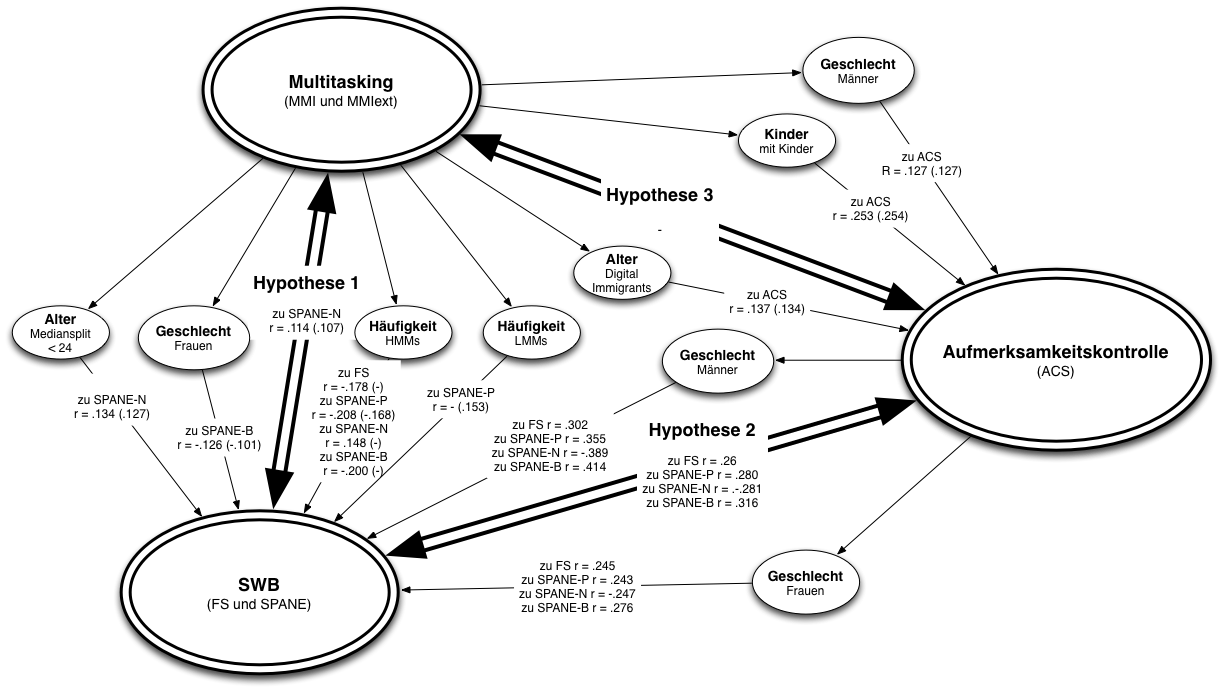
\includegraphics[scale=0.37]{images/grafiken/Zusammenhang_Zusammenfassung_v1.png}
     \caption{Zusammenhang der Variablen}
     \label{pic.ergebniss.zusammenfassung}
\end{figure}




